\documentclass[letter, 12pt]{article}

\usepackage{amsmath,amsthm,amssymb}
\usepackage{fancyhdr}
\usepackage{geometry}
\usepackage{enumerate}
\usepackage{enumitem}
\usepackage{listings}
\usepackage{algorithm}
\usepackage{hyperref}
\usepackage{algorithmic}
\usepackage{eqparbox}
\usepackage{float}
\usepackage{bm}
\usepackage{bbm}
\usepackage{mathtools}
\usepackage{minted}
\usepackage{forest}
\usepackage{cite}

\author{Shengjie Li}
\title{CS 536 : Perceptrons}

\pagestyle{fancy}
\fancyhf{} 
\lhead{Shengjie Li \\ netID: sl1560}
\cfoot{\thepage} 
\renewcommand{\headrulewidth}{1pt}
\renewcommand{\headwidth}{\textwidth}
\renewcommand\algorithmiccomment[1]{%
    \hfill\#\ \eqparbox{COMMENT}{#1}%
}
\newlist{subquestion}{enumerate}{1}
\setlist[subquestion, 1]{label = \alph*)}
\DeclareMathOperator*{\argmax}{arg\,max}
\DeclareMathOperator*{\argmin}{arg\,min}

\setlength\parindent{0pt}

% margin adjustment
\addtolength{\textwidth}{1in}
\addtolength{\oddsidemargin}{-0.5in}
\addtolength{\evensidemargin}{-0.5in}
\addtolength{\topmargin}{-.5in}
\addtolength{\textheight}{1.0in}
\setlength\parindent{0cm}

\begin{document}
    \centerline{\textbf{CS 536 : Perceptrons}}
    \begin{enumerate}
        \item {Show that there is a perceptron that correctly classifies this data. Is this perceptron unique? What is the ‘best’ perceptron for this data set, theoretically?}
        \begin{enumerate}
            \item{Because the class of each data point is only determined by the value of the $ X_k $ feature, it's clear that a perceptron can tell if $ X_k $ is greater than 0 or less than 0.}
            \item{There are infinite perceptrons that can correctly classifies this data. In fact, if we let $ a = max_i(X^i_k), \text{s.t. } Y^i == -1 $ and $ b = min_i(X^i_k), \text{s.t. } Y^i == 1 $, every hyperplane $ a <= x_k <= b $ can correctly classify this data.}
            \item{Theoretically, the best perceptron would be a hyperplane of $ x_k = 0 $. A hyperplane of $ x_k = \frac{a + b}{2} $ can classify the training data very well, but it would fail to generalize for data points with $ X_k \in (a, 0)  \bigcup (0, b). $}
        \end{enumerate}
        
        \item {We want to consider the problem of learning perceptrons from data sets. Generate a set of data of size m = 100
            with $ k = 20, \epsilon = 1 $.}
        \begin{itemize}
            \item {Implement the perceptron learning algorithm. This data is separable, so the algorithm will terminate. How does the output perceptron compare to your theoretical answer in the previous problem?}
            \par{The perceptron I get is: }
            \begin{lstlisting}
w = [[ 0.        ]
    [ 0.02087407]
    [ 0.17257196]
    [-0.55194861]
    [ 0.97983356]
    [-0.85764329]
    [ 0.85379284]
    [-0.89753315]
    [-2.63630402]
    [ 0.3010298 ]
    [ 1.77413824]
    [-1.21897327]
    [-1.87519926]
    [ 0.64459163]
    [ 1.12742088]
    [-0.18981816]
    [ 2.24033418]
    [-0.9949524 ]
    [ 2.1984183 ]
    [ 0.9931059 ]
    [ 7.35863809]]
            \end{lstlisting}
            \par{The first element of my $ \underline{w} $ is the bias unit. The margin of my output perceptron is 0.02223443.}
            \par{While the theoretically best perceptron is:}
            \begin{lstlisting}
w = [[0.]
    [0.]
    [0.]
    [0.]
    [0.]
    [0.]
    [0.]
    [0.]
    [0.]
    [0.]
    [0.]
    [0.]
    [0.]
    [0.]
    [0.]
    [0.]
    [0.]
    [0.]
    [0.]
    [0.]
    [1.]]
            \end{lstlisting}
            \par{The first element of my $ \underline{w} $ is the bias unit. The margin of the theoretically best perceptron is 1.00739826.}
            \par{Thus, my output perceptron has a smaller margin than the theoretically best perceptron, which means it might potentially fail to generalize well in other data sets, which is not a good thing.}
        \end{itemize}
        
        \item {For any given data set, there may be multiple separators with multiple margins - but for our data set, we can effectively control the size of the margin with the parameter $ \epsilon $ - the bigger this value, the bigger the margin of our separator.}
        \begin{itemize}
            \item {For $ m = 100, k = 20 $, generate a data set for a given value of $ \epsilon $ and run the learning algorithm to
                completion. Plot, as a function of $ \epsilon \in [0, 1] $, the average or typical number of steps the algorithm needs to
                terminate. Characterize the dependence.}
            \begin{figure}[H]
            	\centering
            	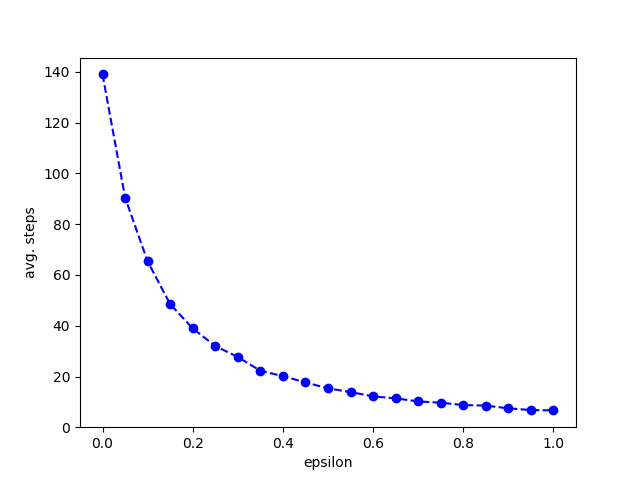
\includegraphics[width=.7\textwidth]{q3.png}
            	\caption{Average number of steps the algorithm needs to terminate}
            \end{figure}
        	\par{The bigger the $ \epsilon $ is, the farther the data points would be separated. It would be easier for the learning algorithm to find a linear separator for larger $ \epsilon $ since the margin is bigger. Thus, with the increase of $ \epsilon $, the average steps of the learning algorithm would first decrease, then start to level out since it would be nearly an instant fit. The shape of the plot looks like half of a hyperbola. }
        \end{itemize}
    
        
        \item {One of the nice properties of the perceptron learning algorithm (and perceptrons generally) is that learning
            the weight vector $ \underline{w} $ and bias value $ b $ is typically independent of the ambient dimension. To see this, consider
            the following experiment:}
        \begin{itemize}
            \item {Fixing $ m = 100, \epsilon = 1 $, consider generating a data set on k features and running the learning algorithm on
                it. Plot, as a function $ k $ (for $ k = 2, \dots , 40 $), the typical number of steps to learn a perceptron on a data
                set of this size. How does the number of steps vary with $ k $? Repeat for $ m = 1000 $.}
            \begin{figure}[H]
	            \centering
	            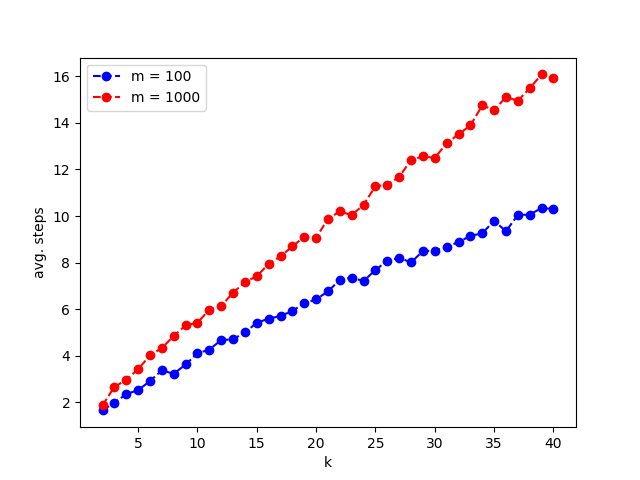
\includegraphics[width=.7\textwidth]{q4-2.png}
	            \caption{Average number of steps the algorithm needs to terminate}
	            \label{q4}
        	\end{figure}
        	\par{As shown in the Fig \ref{q4}, with the increase of $ k $, the average steps the algorithm needs to terminate slowly increases. The increase of average steps is generally linear.}
        \end{itemize}
        
        \item {As shown in class, the perceptron learning algorithm always terminates in finite time - if there is a separator.
            Consider generating non-separable data in the following way: generate each $ X_1 , \dots , X_k $ as i.i.d. standard
            normals $ N (0, 1) $. Define Y by \[ Y = \begin{cases}
            +1 & \text{if } \sum_{i=1}^{k}X_i^2 \ge k \\
            -1 & \text{else}.
            \end{cases} \]}
        \par{For data defined in this way, there is no universally applicable linear separator.}
        \par{For $ k = 2, m = 100 $, generate a data set that is not linearly separable. (How can you verify this?) Then run
            the perceptron learning algorithm. What does the progression of weight vectors and bias values look like over
            time? If there is no separator, this will never terminate - is there any condition or heuristic you could use to
            determine whether or not to terminate the algorithm and declare no separator found?}
        \begin{figure}[H]
	        \centering
	        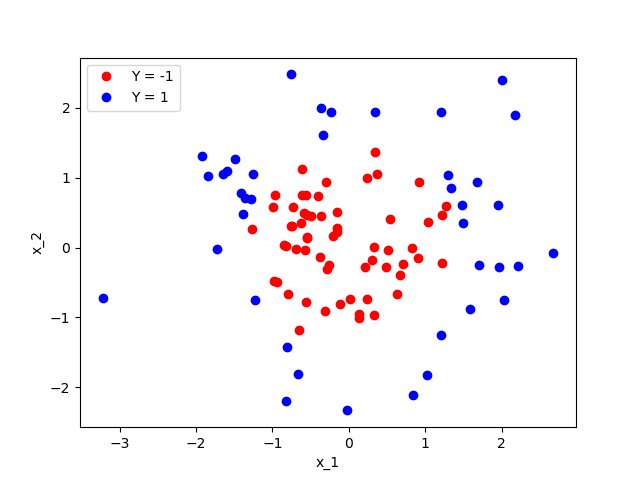
\includegraphics[width=.7\textwidth]{q5.png}
	        \caption{Data set}
	        \label{q5}
	    \end{figure}
    	\par{There are several methods to verify if the data is linearly separable.}
    	\begin{enumerate}
    		\item{If the data has intersecting convex hulls, then the data is not linearly separable \cite{holmes}. But this is hard to tell if the data is high dimensional.}
    		\item{If the learning algorithm runs over a certain number of steps, then the data is not linearly separable.}
    	\end{enumerate}
   		\par{Since the data is only 2-dimensional, I am going to plot my data here.}
    	\par{As Fig \ref{q5} shows, there is clearly no linear separator that can separate this data. }
    	\begin{figure}[H]
    		\centering
    		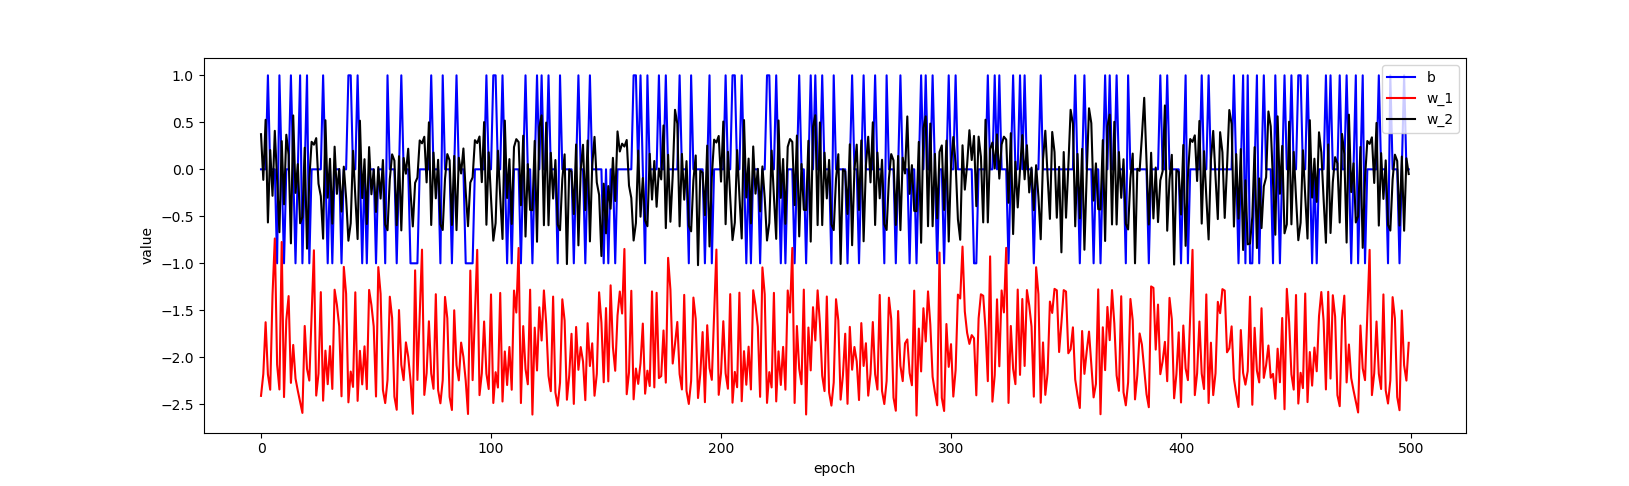
\includegraphics[width=\linewidth]{q5-2.png}
    		\caption{The progression of weight vectors and bias values}
    		\label{q5-2}
    	\end{figure}
    	\par{From the Fig \ref{q5-2} above we can see that the values are always swaying.}
    	\par{I propose a heuristic:}
    	\begin{enumerate}
    		\item {Set the max epoch to be a large enough number, say 10000.}
    		\item {Record the number of misclassified data points, say it's $ p $.}
    		\item {Update max epoch as $ min(\textit{max\_epoch}, \textit{current\_epoch} + 2 * p) $}
    	\end{enumerate}
    	\par{If the program runs over the \textit{max\_epoch}, I would say there's no separator for the data.}
    \end{enumerate}

	\bibliography{mybib}{}
	\bibliographystyle{plain}
\end{document}
